\documentclass{acm_proc_article-sp}
\usepackage{mdwlist}
\usepackage{xcolor}
\usepackage[colorlinks,
  linkcolor=black,
  anchorcolor=black,
  urlcolor=black,
  citecolor=black
  ]{hyperref}

\begin{document}

\title{Experiment Report: Indexing Images\\
for Content Based Retrieval}

\numberofauthors{3} 
\author{
\alignauthor
Dang Fan\titlenote{Student ID: 2009013215}\\
       \affaddr{School of Software}\\
       \affaddr{Tsinghua University}\\
       \email{\href{mailto:dangf09@gmail.com}{dangf09@gmail.com}}
\alignauthor
Ding Peng\titlenote{Student ID: 2009013219}\\
       \affaddr{School of Software}\\
       \affaddr{Tsinghua University}\\
       \email{\href{mailto:dingpeng09@gmail.com}{dingpeng09@gmail.com}}
\alignauthor
Wang Shuhao\titlenote{Student ID: 2009013229}\\
       \affaddr{School of Software}\\
       \affaddr{Tsinghua University}\\
       \email{\href{mailto:shudiwsh2009@gmail.com}{shudiwsh2009@gmail.com}}
}

\maketitle
\begin{abstract}
The aim of this paper is to provide a report of an experiment using image features to index and search images by content. It presents the main method of features extraction based on histogram, the comparison of effectiveness and relevance by varing the number and type of features.
%, and the approach to improve the performance of R-tree.
\end{abstract}

\category{I.4.7}{Image Processing and Computer Vision}{Feature Measurement}
\category{H.2.8}{Database Management}{Database Applications}

\terms{Experimentation}

\keywords{image index, histogram, r-tree}

\section{Outline}
\subsection{Experimental System}
This experimental system is written in Python. However, the imaging package (Python Imaging Library) and the core of R-tree package (libspatialindex) are written in C/C++.

The Python Imaging Library (PIL)\cite{website:PIL} can be downloaded from \texttt{\url{http://effbot.org/downloads/Imaging-1.1.7.tar.gz}}. Notice that it is required to install libjpeg first in order to deal with JPEG files according to the installation instruction.

The R-tree libraries are located at \texttt{/experiment1/libs/}. libspatialindex (\texttt{spatialindex-src-1.7.1.tar.gz})\cite{website:si} is a library to provide a framework that supports spatial indexing methods, which can be found at \texttt{\href{http://libspatialindex.github.com/}{http://libspatialindex. github.com/}}. Rtree (\texttt{Rtree-0.7.0.tar.gz})\cite{website:rtree} is a ctypes Python wrapper of libspatialindex, which can be found at \texttt{\url{http://toblerity.github.com/rtree/}}. In this experiment, we modified these two libraries to achieve the requirement of this experiment, including counting the number of node access.
% and adjustment of parameters of Rtree.

This experimental system consist of 4 files:

\begin{itemize*}
  \item \texttt{ImageFeatureExtractorV1.py}
  \item \texttt{ImageFeatureExtractorV2.py}
  \item \texttt{Queries.py}
  \item \texttt{Main.py}
\end{itemize*}

The first two files are implementations of two different approaches of color histogram features, which is defined in section~\ref{feature definition}.

The third file is used to generate the number of node access with respect to the various number of features and the number of data objects inserted. It also generates the correctness rate, which is defined in section~\ref{problem3}.

The last file is a program that provided an interface for querying by example.

A README file (\texttt{/experiment1/programs/README}) is provided to show how to run these programs.

For the first three files, we have got the test result put in the directory \texttt{/experiment1/data/}. The directory \texttt{attempt1} contains the result generated by the program \texttt{ImageFeatureExtractorV1.py}. The directory \texttt{attempt2} contains the result generated by the program \texttt{ImageFeatureExtractorV2.py}. The directory \texttt{moment} contains the features and imagelist provided by the project. We strongly recommend that you use the data generated by us, for the reason that running these programs may be extremely slow.

\subsection{Definitions of the features}
\label{feature definition}
As the project suggested, we use color histogram as the feature. In this experiment, we make two approaches to generate vector-form features.

In the first approach, we generate the color histogram vector of red, green and blue separately, with a 256-ranked vector of each color, by counting the number of pixels in respect to the bin. After that, we simply concatenate the vectors and get a histogram vector of rank 768 (256 $\times$ 3). Then we divide it into $D$ parts, where $D$ is the dimension we need, and sum up each part. For instance, a one-pixel red image has only one pixel with rgb=(255, 0, 0). Thus, three 1s show up in the histogram vector, located at 255, 256 and 512. If we need a 4-dimension vector, then it produces (0, 2, 1, 0). The program \texttt{ImageFeatureExtractorV1.py} implements this approach.

In the second approach, we generate the color histogram vector according to the method provided in this class. That is a histogram of an image is produced first by discretization of the colors in the image into a number of bins, and counting the number of image pixels in each bin. An example can be found at Wikipedia \cite{website:wikihist}. The program \texttt{ImageFeatureExtractorV2.py} implements this approach.

\section{Main Results}
\subsection{Problem 1}
In this problem, we tested the performance of R-tree based query processing in terms of node access number. For each approach described in section~\ref{feature definition}, we used features with dimension of 4, 8, 12, 16, 20, 27 and 64, and data objects inserted with number of 200, 400, ..., 5600. In each test, we did random nearest queries 5000 times.

Figure~\ref{fig:p2a1} and~\ref{fig:p2a2} demonstrates the average node access number per query with the corresponding parameter in approach 1 and 2.

\begin{figure}
\centering
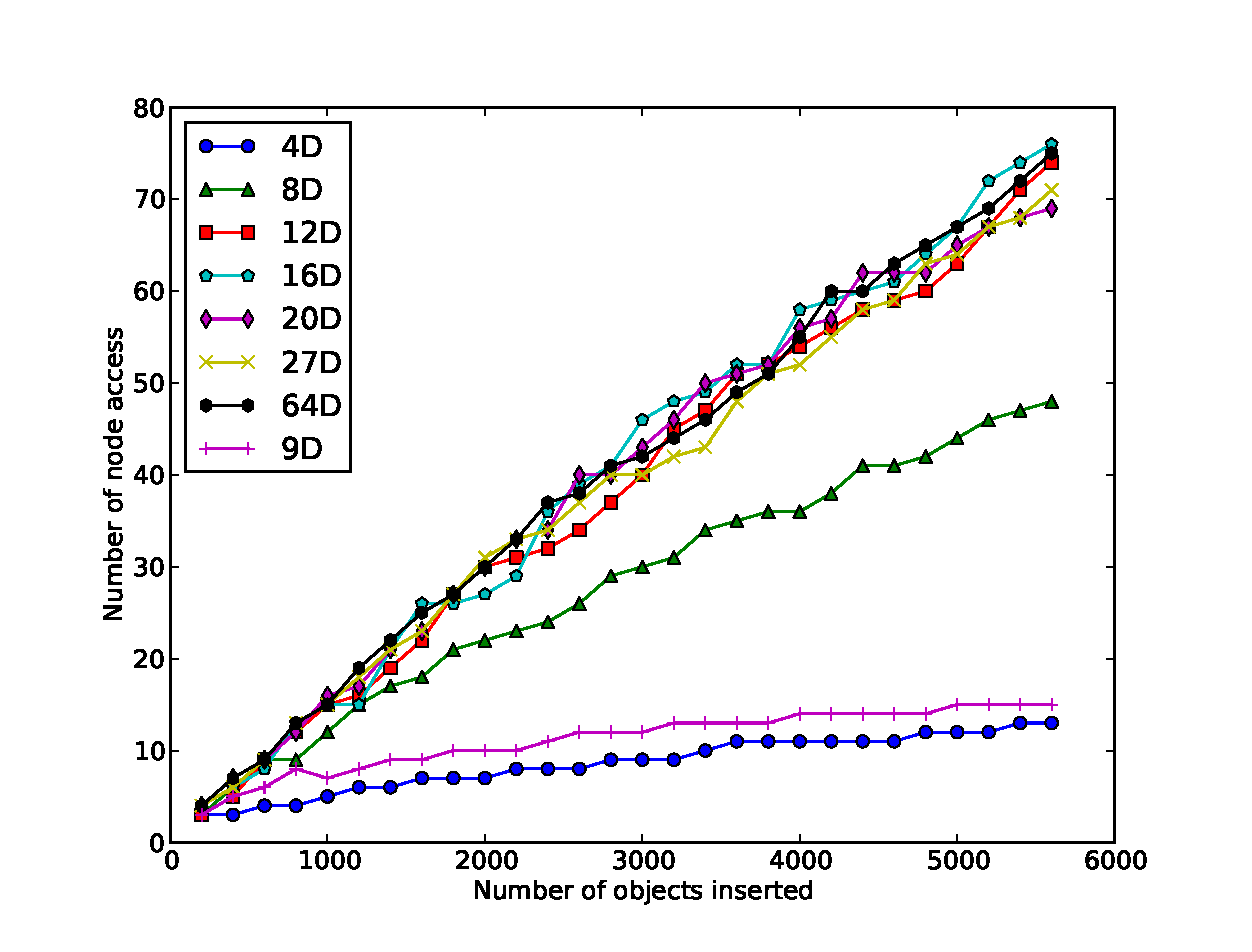
\epsfig{file=p2a1.eps, width=0.5\textwidth}
\caption{The average node access number per query in approach 1}
\label{fig:p2a1}
\end{figure}

\begin{figure}
\centering
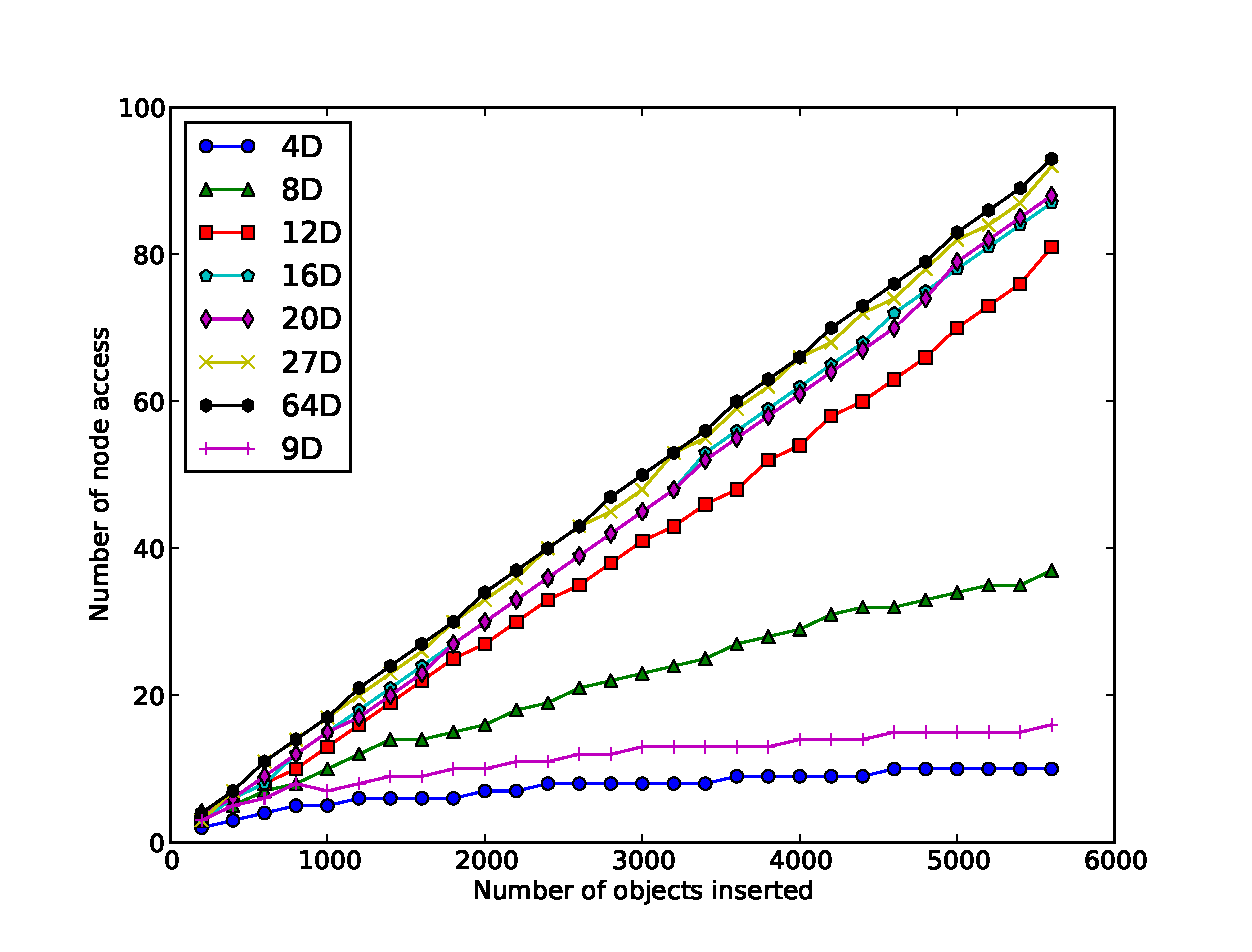
\epsfig{file=p2a2.eps, width=0.5\textwidth}
\caption{The average node access number per query in approach 2}
\label{fig:p2a2}
\end{figure}

\subsection{Problem 2}
In this problem, we tested the performance of the features provided by this project (color moment feature). Then compare it to the features that we extracted. The results are shown in figure~\ref{fig:p2a1} and~\ref{fig:p2a2}, which are similar with the figures in problem 1. Note that the result of color moment feature is the line with label \textit{9D}.

\subsection{Problem 3}
\label{problem3}
In this problem, we used both the color histogram features and color moment features to test the relevance. We randomly chose a image, and searched its neareast 10, 20, 30, ..., 100 images, then count the images that are in the same category to the sample and calculate the correctness rate. We did this 100 times and use the average rate as the result.

The results of approach 1 and 2 are shown in figure~\ref{fig:p3a1} and~\ref{fig:p3a2}.

\begin{figure*}
\centering
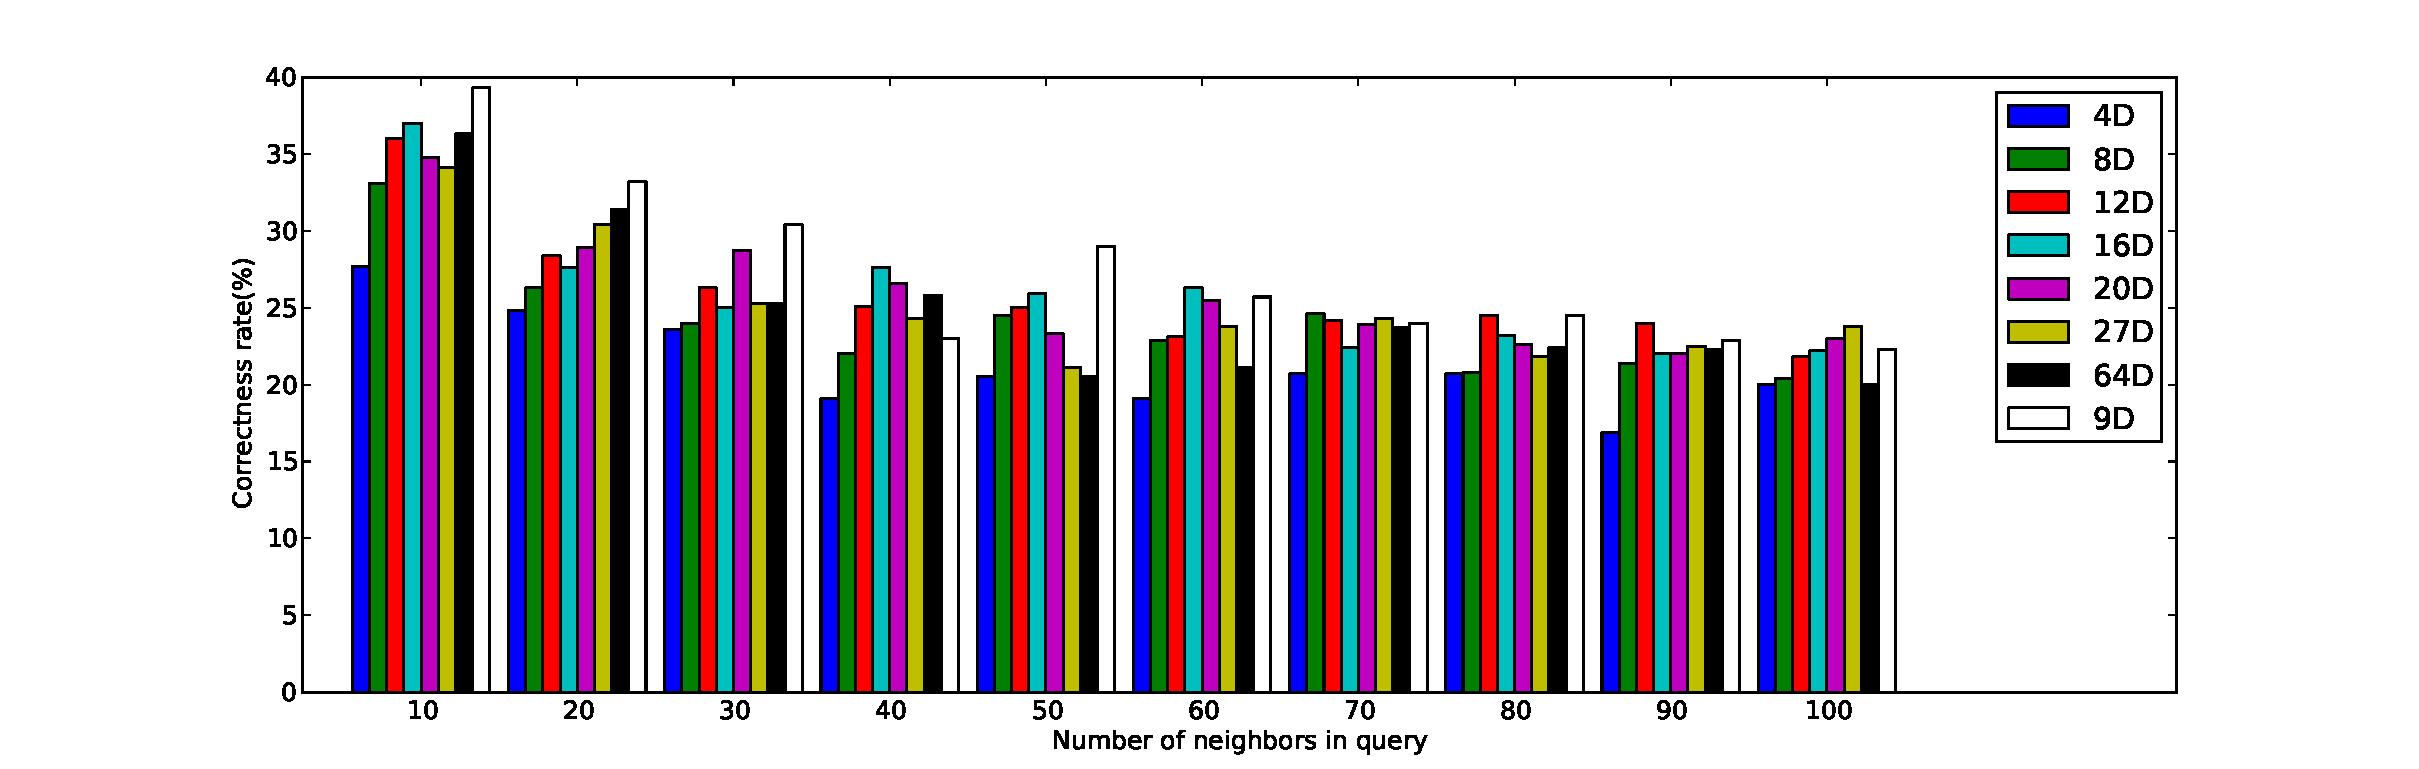
\includegraphics[width=0.8\textwidth]{p3a1.pdf}
\caption{The correctness rate of approach 1}
\label{fig:p3a1}
\end{figure*}

\begin{figure*}
\centering
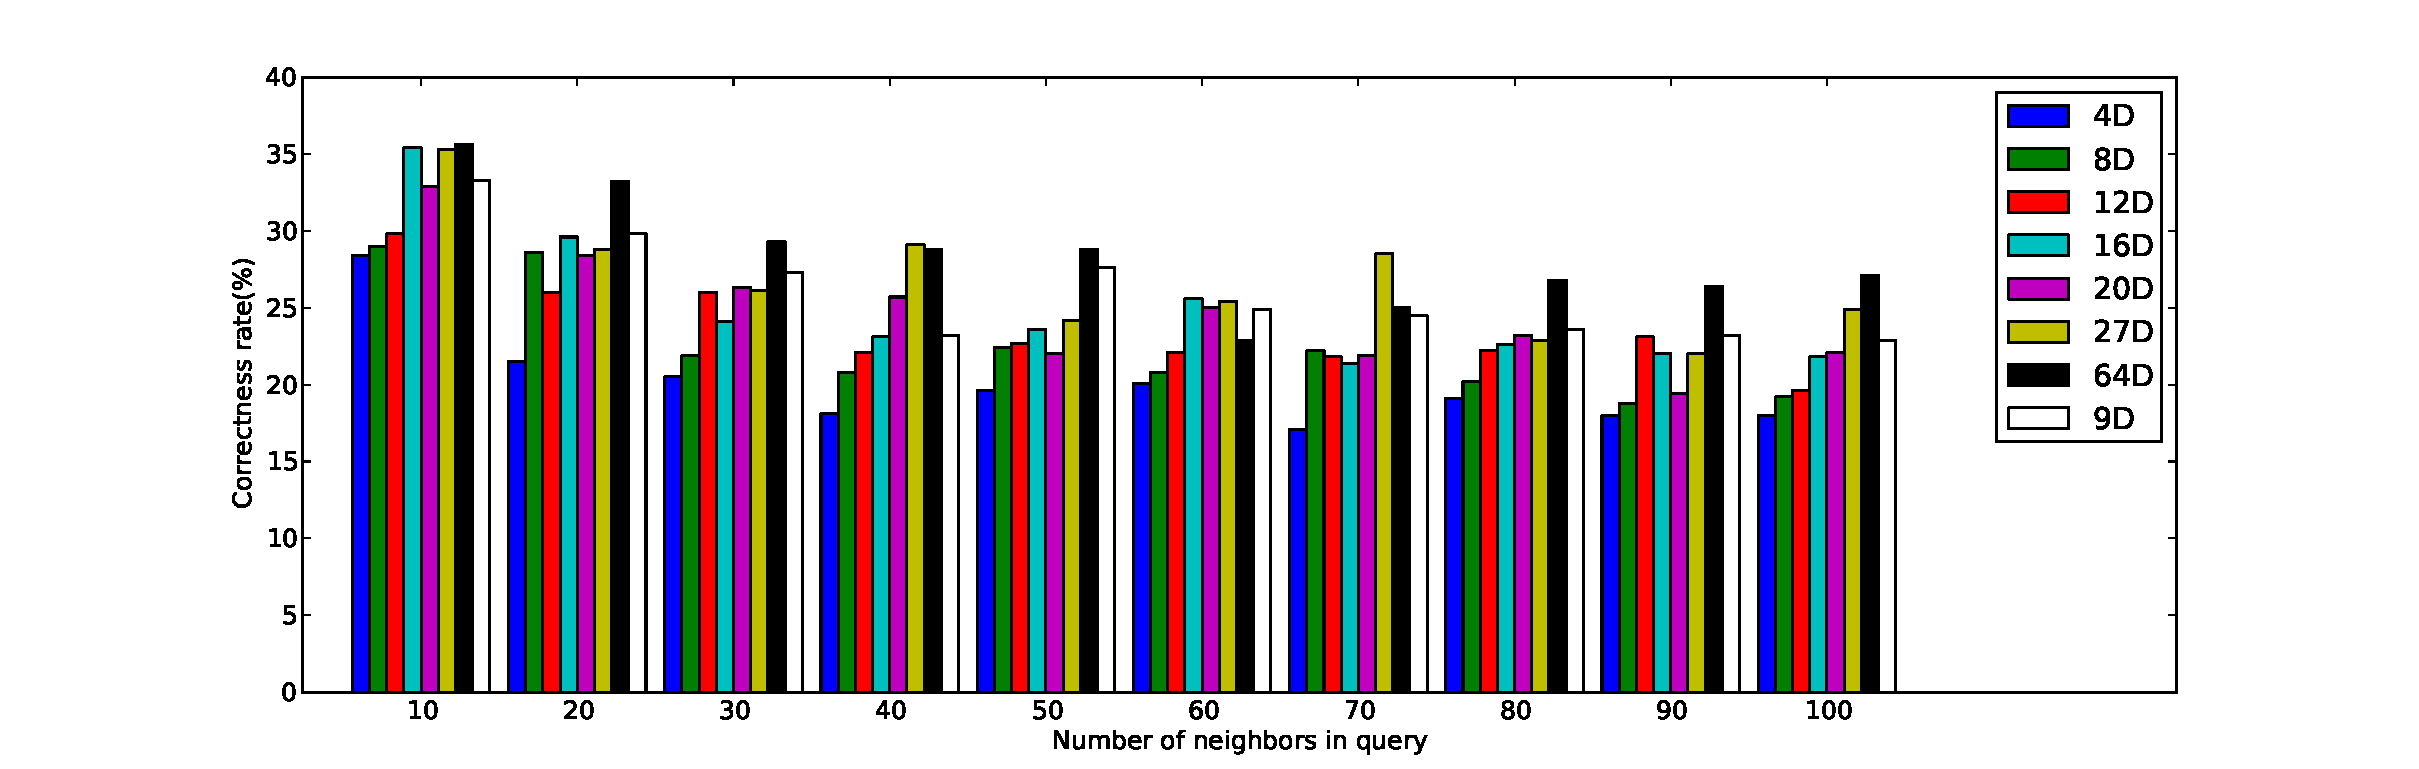
\includegraphics[width=0.8\textwidth]{p3a2.pdf}
\caption{The correctness rate of approach 2}
\label{fig:p3a2}
\end{figure*}

\section{Analysis and Conclusions}
\subsection{Performance}
In both approaches, we find that the number of node access increases dramatically with the increase of the dimension. Especially with color histogram features extracted by us, when the dimension is greater than 8, the number of node access is pretty high. 

On the other hand, we find that the number of node access and the number of objects inserted are approximately in linear relationship.

When compared to the color moment feature (the \textit{9D} line), we find that its performance is pretty good. From the figure~\ref{fig:p2a1} and~\ref{fig:p2a2}, we can see that the number of node access with 8 dimension (color histogram feature) is much higher than that with 9 dimension (color moment feature).

Based on the analysis above, we can draw the conclusion that three factors affect the performance of R-tree:

\begin{itemize*}
  \item The dimension of data object.

  The higher the dimension is, the more node access it requires.

  \item The number of data objects inserted.

  The more data objects are inserted, the more node access it requires.

  \item The content of data object.

  Color moment feature in 9 dimension has better performance than color histogram feature in 8 dimension, thus the content of data objects also affects the performance of R-tree. We guess the more precise factor is how well the data objects are linear independent. Unfortunately, we have not figure out a proper way to prove it.
\end{itemize*}

\subsection{Relevance}
Figure~\ref{fig:p3a1} and~\ref{fig:p3a2} demonstrate the relevance or the correctness of each approach.

In the first approach, the color moment feature is almost the best, reached nearly 40\% correctness rate in 10 nearest neighbors search. However, we also notice that, the histogram feature is not so bad, especially when the dimension is greater than or equal to 12. The result of approach can be accepted due to it is close to the color moment feature.

In the second approach, we find that this histogram feature works much better. In most cases, it is more precise than color moment feature with dimension above 20.

The conclusion is that the relevance is affected by:

\begin{itemize*}
 \item The feature type.

 The color histogram feature in approach 2 has the best correctness rate.

 \item The dimension of features.

 The higher the dimension is, the more correct the result is.
\end{itemize*}

\subsection{Summary}
Based on the analysis above, it is obvious to see that it is difficult to balance the performance and the relevance. To achieve better performance, we need to reduce the dimension. However, higher dimension feature has better correctness. Thus, we have to choose a proper feature (considering its type and dimension) based on the actual requirement.

\section{Acknowledgments}
Thanks to Mr. Jin for being such good guider for us. He had given us appropriate example and knowledge in order to make us understand more about this project.


\bibliographystyle{plain}
\bibliography{sigproc}

%\balancecolumns

\end{document}
